\documentclass[letterpaper,11pt]{article}
\renewcommand{\normalsize}{\fontsize{9pt}{11pt}\selectfont}

\usepackage{latexsym}
\usepackage[empty]{fullpage}
\usepackage{titlesec}
\usepackage{marvosym}
\usepackage[usenames,dvipsnames]{color}
\usepackage{verbatim}
\usepackage{enumitem}
\usepackage[hidelinks]{hyperref}
\usepackage{fancyhdr}
\usepackage[english]{babel}
\usepackage{tabularx}
\usepackage{graphicx}
\input{glyphtounicode}

\pagestyle{fancy}
\fancyhf{} % clear all header and footer fields
\fancyfoot{}
\renewcommand{\headrulewidth}{0pt}
\renewcommand{\footrulewidth}{0pt}

% Adjust margins
\addtolength{\oddsidemargin}{-0.5in}
\addtolength{\evensidemargin}{-0.5in}
\addtolength{\textwidth}{1in}
\addtolength{\topmargin}{-.5in}
\addtolength{\textheight}{1.0in}

\urlstyle{same}

\raggedbottom
\raggedright
\setlength{\tabcolsep}{0in}

% Sections formatting
\titleformat{\section}{
  \vspace{-4pt}\scshape\raggedright\large
}{}{0em}{}[\color{black}\titlerule \vspace{-5pt}]

% Ensure that generate pdf is machine readable/ATS parsable
\pdfgentounicode=1

%-------------------------
% Custom commands
\newcommand{\resumeItem}[2]{
  \item\small{
    \textbf{#1}{: #2 \vspace{-2pt}}
  }
}

\newcommand{\resumeSubheading}[4]{
  \vspace{-1pt}\item
    \begin{tabular*}{0.97\textwidth}[t]{l@{\extracolsep{\fill}}r}
      \textbf{#1} & #2 \\
      \textit{\small#3} & \textit{\small #4} \\
    \end{tabular*}\vspace{-5pt}
}

\newcommand{\resumeSubItem}[2]{\resumeItem{#1}{#2}\vspace{-4pt}}

\renewcommand{\labelitemii}{$\circ$}

\newcommand{\resumeSubHeadingListStart}{\begin{itemize}[leftmargin=*]}
\newcommand{\resumeSubHeadingListEnd}{\end{itemize}}

%-------------------------------------------
%%%%%%  CV STARTS HERE  %%%%%%%%%%%%%%%%%%%%%%%%%%%

\begin{document}

%----------HEADING-----------------
\begin{minipage}[t]{0.83\textwidth}
\begin{tabularx}{\textwidth}{X r}
  \textbf{\Large Harith Iduwara} \\
  {}\\
  \href{https://www.linkedin.com/in/iduwara/}{LinkedIn} $|$ \href{https://github.com/harithiduwara}{GitHub} \\
  Email: \href{mailto:contactharith@gmail.com}{contactharith@gmail.com}
\end{tabularx}
\end{minipage}
\hfill
\begin{minipage}[t]{0.15\textwidth}
  \begin{tabular}{r}
    % Add a file named photo.jpg alongside this file to include a headshot
    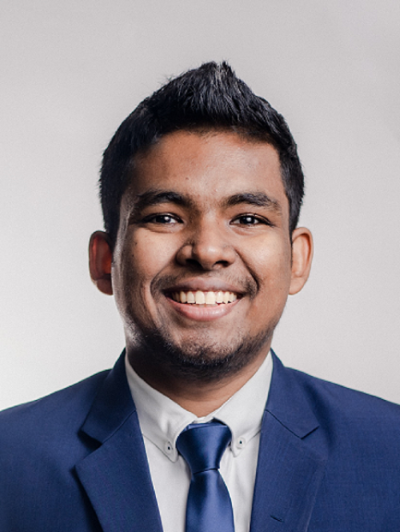
\includegraphics[width=1.9cm]{photo.jpg}
  \end{tabular}
\end{minipage}

%-----------EXPERIENCE-----------------
\section{Experience}
\resumeSubHeadingListStart

  \item
  \textbf{Software Engineer} \hfill Jan 2024 -- Present \\
  \textit{London Stock Exchange Group (LSEG) Technologies}, Malabe, Sri Lanka
  \begin{itemize}[leftmargin=*, topsep=2pt]
    \item \textbf{FXAll -- Buyside8 Team} \hfill Jun 2025 -- Present
    \begin{itemize}[leftmargin=*]
        \item Designed and executed test plans for Fixing Settings and Resting Orders workflows, covering scenario creation, validation, edge-case analysis, and automation integration.
        \item Investigated and resolved regression failures identified in daily in-sprint test reports for releases 4.0.11 and 4.0.12, improving overall stability and reducing recurring defects.
        \item Performed extensive UI, API, and FIX message testing to validate order lifecycle behavior and ensure functional accuracy across FXAll workflows.
    \end{itemize}

    \item \textbf{CMQA -- Tools Team} \hfill Jan 2024 -- Jun 2025
    \begin{itemize}[leftmargin=*]
        \item Developed and enhanced the Model-Based Testing (MBT) tool to validate reference data and FX matching systems, improving accuracy and maintainability.
        \item Analyzed and developed features for the FX Reconciliation Tool, enhancing reliability and reducing reconciliation gaps.
        \item Contributed to the FX Credit GUI Test Automation framework using Java, Cucumber, and Playwright to increase automation stability and reduce manual QA workload.
        \item Developed and maintained functionality in the Fortress2 testing tool using BDD practices to streamline cross-team collaboration.
        \item Built utility scripts to improve performance and workflow efficiency across MBT, Sailfish, and Reconciliation systems.
    \end{itemize}
  \end{itemize}
  \small{\textbf{Technologies:} Python, Java, Bash, Playwright, C++, Cucumber, FIX Protocol, API Testing}

  \item \vspace{0.5em}
  \textbf{Software Engineering Intern} \hfill Nov 2022 -- Nov 2023 \\
  \textit{London Stock Exchange Group (LSEG) Technologies}, Malabe, Sri Lanka
  \begin{itemize}[leftmargin=*, topsep=2pt]
    \item \textbf{LSEG Surveillance Analytics} \hfill May 2023 -- Nov 2023
    \begin{itemize}[leftmargin=*]
        \item Researched and evaluated the feasibility of upgrading Apache Atlas from 2.1.0 to 2.3.0; successfully deployed and configured Atlas in an AWS EC2 environment.
        \item Contributed to the development of the Configuration Module within the LSEG Surveillance Analytics platform.
    \end{itemize}

    \item \textbf{FX Surveillance Postgres Cutover} \hfill Nov 2022 -- May 2023
    \begin{itemize}[leftmargin=*]
        \item Supported the migration of the FX Surveillance system's database layer from Oracle to Postgres.
        \item Engaged in low-level debugging and system performance monitoring using C++, SQL, Bash, GDB, and Sysguard.
    \end{itemize}
  \end{itemize}
  \small{\textbf{Technologies:} Python, Postgres, Apache Atlas, Spark, AWS (EC2, S3), C++, SQL, Bash, GDB, Sysguard}

\resumeSubHeadingListEnd

%-----------ACHIEVEMENTS---------------
\section{Achievements}
\begin{itemize}[leftmargin=*, itemsep=-2pt]
  \item \href{https://www.linkedin.com/posts/iduwara_nbqsa-srilanka-ict-activity-6994599226454282240-XTe1}{\textbf{National ICT Awards (NBQSA)} -- Silver, Tertiary Student Technology} | 2022
  \item Represented the \textbf{LSEG Cricket Team} at the Mercantile Cricket Tournament | 2022 -- Present
  \item Represented the \textbf{D. S. Senanayake College} Cricket Team | 2012 -- 2016
  \item Sri Lankan \textbf{Physics Olympiad} Competition -- Merit | 2017
  \item Videographer, National Showcasing Team, \textbf{AIESEC Sri Lanka} | 2021 -- 2022
  \item Committee Member, Student Council, Wisdom Business Academy | 2018
  \item Marketing Member, AIESEC Colombo Central | 2021
  \item \textbf{Head of Photography}, Pahasara UCSC | 2020 -- 2022
\end{itemize}

%-----------PROJECTS-----------------
\section{Projects}
\resumeSubHeadingListStart
  \resumeSubItem{SpeechAssist}
    {A mobile and web-based solution for treating stammering using DAF and FAF methods. Built with ReactJS. Won Silver at NBQSA 2022.}
  \resumeSubItem{Wadak}
    {An online marketplace for freelancers, designed and implemented using HTML, CSS, and PHP without the use of any framework.}
  \resumeSubItem{TradingView Indicator}
    {An indicator using Pine Script to visualise EMAs on TradingView charts.}
  \resumeSubItem{TG-DEX}
    {A TG-DEX trader built with the Telegram API and Solana SDK in Python to trade on Solana DEXes as a hobby project.}
  \resumeSubItem{Algorithmic Bots}
    {Algorithmic bots that trade currencies across different market conditions. Strategies currently run in 3Commas, with AI features planned for the future.}
  \resumeSubItem{Handwritten Character Recogniser}
    {Used thresholding, contour detection, and feature extraction to preprocess and analyze handwritten characters without using machine learning techniques.}
\resumeSubHeadingListEnd

%-----------EDUCATION-----------------
\section{Education}
\resumeSubHeadingListStart
  \resumeSubheading
    {University of Colombo School of Computing}{Colombo, Sri Lanka}
    {Bachelor of Science in Computer Science | Second Class Upper Division}{2019 -- 2023}
  \resumeSubheading
    {D. S. Senanayake College}{Colombo, Sri Lanka}
    {GCE Advanced Levels; Combined Maths (A), Chemistry (A), Physics (B)}{Aug 2018}
  \resumeSubheading
    {D. S. Senanayake College}{Colombo, Sri Lanka}
    {GCE Ordinary Levels; 8 A's, 1 B}{Dec 2014}
\resumeSubHeadingListEnd

%-----------TECHNICAL SKILLS-----------------
\section{Technical Skills}
\resumeSubHeadingListStart
  \item \textbf{Languages:} C++, Python, Java, SQL
  \item \textbf{Web Development:} PHP, JavaScript, HTML, CSS
  \item \textbf{Technologies:} AWS, Jenkins
\resumeSubHeadingListEnd

%-----------REFERENCES---------------
% References available upon request.

\end{document}
